
\chapter{Reduction of Spatial Convolution by FFT\label{chpt:fft-spatial}}

As presented in section \ref{chpt:mdft}, to complete the minimization
process of MDFT, we need to evaluate the excess functional as well
as its gradient:
\begin{equation}
\mathcal{F}_{\mathrm{exc}}=-\frac{\beta^{-1}}{2}\int\mathrm{d}\mathbf{r_{1}}\mathrm{d}\mathbf{r_{2}}\mathrm{d}\mathbf{\Omega_{1}}\mathrm{d}\mathbf{\Omega_{2}}\Delta\rho(\mathbf{r_{1}},\mathbf{\Omega_{1}})\Delta\rho(\mathbf{r_{2}},\mathbf{\Omega_{2}})c(\mathbf{r}_{12},\mathbf{\Omega_{1}},\mathbf{\Omega_{2}})\label{eq:fexc}
\end{equation}
\begin{equation}
\gamma(\mathbf{r_{1}},\mathbf{\Omega_{1}})=-\beta^{-1}\int\mathrm{d}\mathbf{r_{2}}\mathrm{d}\mathbf{\Omega_{2}}\Delta\rho(\mathbf{r}_{2},\mathbf{\Omega}_{2})c(\mathbf{r}_{12},\mathbf{\Omega}_{1},\mathbf{\Omega}_{2})\label{eq:gamma}
\end{equation}

To evaluate the gradient $\gamma$ for each $\mathbf{(r},\mathbf{\Omega})$,
$N\equiv N_{\mathbf{r}}N_{\mathbf{\Omega}}$ function evaluations
(FE) are required, the total number of FE is thus $N^{2}=O(N^{2})$,
which, with typically $N_{\mathbf{r}}=64^{3}$ and $N_{\mathbf{\Omega}}=50\sim100$,
is far too costly for current computing technology. For this reason,
Fourier transform is used to treat the spatial convolution in eq.
(\ref{eq:gamma}).

A convolution
\begin{equation}
h(x_{1})\equiv f(x_{2})\otimes g(x_{2})\equiv\int_{a}^{b}f(x_{2})g(x_{1}-x_{2})dx_{2}\label{eq:convolution-1}
\end{equation}
has the property that
\begin{equation}
\mathfrak{F}[h(x_{1})]=\mathfrak{F}[f(x_{2})]\mathfrak{F}[g(x_{2})]\label{eq:convolution-2}
\end{equation}
$\mathfrak{F}$ being the Fourier transform (FT) operation \textcolor{red}{(Attention
d'avoir bien défini les FFT 3D avant)}. As $\mathbf{r_{12}}=\mathbf{r_{1}}-\mathbf{r_{2}}$,
eq. (\ref{eq:gamma}) is a 3D convolution, which leads to 
\begin{equation}
\hat{\gamma}(\mathbf{k},\mathbf{\Omega_{1}})=-\beta^{-1}\int\mathrm{d}\mathbf{\Omega_{2}}\Delta\hat{\rho}(\mathbf{k},\mathbf{\Omega_{2}})\hat{c}(\mathbf{k},\mathbf{\Omega_{1}},\mathbf{\Omega_{2}})\label{eq:gamma-k}
\end{equation}

Thus the integral $\int\mathrm{d}\mathbf{r_{2}}$ in eq. (\ref{eq:gamma})
is transformed into a simple product in eq. (\ref{eq:gamma-k}). To
get $\hat{\gamma}(\mathbf{k},\mathbf{\Omega_{1}})$ with given $\Delta\hat{\rho}(\mathbf{k},\mathbf{\Omega_{2}})$,
only $N_{\mathbf{r}}N_{\mathbf{\Omega}}^{2}$ FE are needed. To this
computational cost should be added the transform from $\Delta\rho(\mathbf{r},\mathbf{\Omega})$
to $\Delta\hat{\rho}(\mathbf{k},\mathbf{\Omega})$ and the backward
transform from $\hat{\gamma}(\mathbf{k},\mathbf{\Omega})$ to $\gamma(\mathbf{r},\mathbf{\Omega})$
which are both of order $N_{\mathbf{\Omega}}\cdot O(N_{\mathbf{r}}\log_{2}N_{\mathbf{r}})$,
due to the properties of Fast Fourier Transforms (FFT). The total
number of FE is thus reduced from quadratic complexity $O(N_{\mathbf{r}}^{2}N_{\mathbf{\Omega}}^{2})$
to $N_{\mathbf{r}}N_{\mathbf{\Omega}}^{2}+2N_{\mathbf{\Omega}}\cdot O(N_{\mathbf{r}}\log_{2}N_{\mathbf{r}})=O(N_{\mathbf{r}}\log_{2}N_{\mathbf{r}}N_{\mathbf{\Omega}}^{2})$.
As the total number of spatial grid $N_{\mathbf{r}}$ is of magnitude
$10^{5}\sim10^{6}$, this procedure, which is mathematically equivalent
to the direct evaluation (\ref{eq:gamma}), gives a great advantage
in terms of computational efficiency (figure \ref{fig:order-of-growth}
in section \ref{chpt:introduction}).

Once $\gamma(\mathbf{r},\mathbf{\Omega})$ is obtained by inverse
Fourier transform of $\gamma(\mathbf{r},\mathbf{\Omega})$, the excess
functional can be calculated as:
\begin{equation}
\mathcal{F}_{\mathrm{exc}}[\rho(\mathbf{r},\mathbf{\Omega})]=\frac{1}{2}\int\mathrm{d}\mathbf{r}\mathrm{d}\mathbf{\Omega}\Delta\rho(\mathbf{r},\mathbf{\Omega})\gamma(\mathbf{r},\mathbf{\Omega})
\end{equation}

It should be pointed out that the direct correlation function (DCF),
$\hat{c}(\mathbf{k},\mathbf{\Omega}_{1},\mathbf{\Omega}_{2})$, used
as an input data in eq. (\ref{eq:gamma-k}) is very memory-costly.
For instance, with a normal setting with $64^{3}$ spatial grid and
a Lebedev quadrature of order 2 (14 angles for $\Theta$ and $\Phi$),
and 3 $\Psi$-angles, even if the DCF is stocked in simple precision,
it takes $64^{3}\times42^{2}\times4\,\mathrm{bytes}=1.76\mathrm{GB}$,
and for a Lebedev quadrature of order 5 and correspondingly 5 $\Psi$-angles,
it takes $64^{3}\times250^{2}\times4\,\mathrm{bytes}=65.5\mathrm{GB}$.
As a normal PC has only 4 to 16 GB of RAM, it can cause a memory leak.
Therefore, two strategies are developed to reduce the storage of the
DCF.

\section{Using intermolecular DCF}

\textcolor{red}{(In the previous work, the interpolation has been
done with $\mathbf{\Omega}\equiv(\Theta,\Phi)$. Here, we discuss
the case of full 3 Euler angles $\mathbf{\Omega}\equiv(\Theta,\Phi,\Psi)$.
: To be put somewhere else.)}

The first strategy aims to work in the so-called intermolecular frame
described in fig. \ref{fig:coordinate_systems} for which, in $\mathbf{r}$-space,
the $z$ axis is oriented along the vector $\mathbf{r_{12}}=\mathbf{r_{2}}-\mathbf{r_{1}}$,
or in $\mathbf{k}$-space is oriented along the vector $\mathbf{k}$.
In the latter case, an orientation $\mathbf{\Omega}\equiv(\Theta,\Phi,\Psi)$
in laboratory frame become $\boldsymbol{\omega}\equiv(\theta,\phi,\psi)$
in intermolecular frame. 

To store the DCF in the intermolecular coordinates system, it can
be defined as $\hat{c}(k,\boldsymbol{\omega_{1}},\boldsymbol{\omega_{2}})$,
where $(\boldsymbol{\omega_{1}},\boldsymbol{\omega_{2}})\equiv(\cos\theta_{1},\cos\theta_{2},\phi,\psi_{1},\psi_{2})$
and $k$ is always oriented along the $z$ axis (figure \ref{fig:coordinate_systems})
such that only 6 variables are needed instead of 9 for $\hat{c}(\mathbf{k},\mathbf{\Omega}_{1},\mathbf{\Omega}_{2})$,
and the storage is considerably reduced. The transform from $\hat{c}(k,\boldsymbol{\omega_{1}},\boldsymbol{\omega_{2}})$
to $\hat{c}(\mathbf{k},\mathbf{\Omega_{1}},\mathbf{\Omega_{2}})$
relies on the correspondence $\boldsymbol{\omega}(\mathbf{k},\mathbf{\Omega})\equiv(\cos\theta,\phi,\psi)$,
which can be pre-calculated as a table of data.

\selectlanguage{english}%
\begin{figure}[h]
\begin{centering}
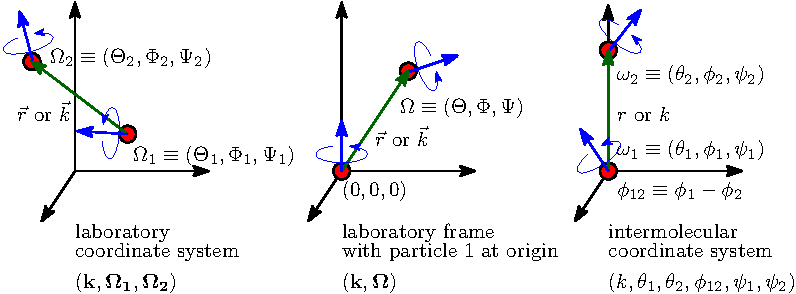
\includegraphics{_figure/coordinate_system}
\par\end{centering}
\caption{\foreignlanguage{american}{Molecules 1 and 2 in different coordinate systems\foreignlanguage{english}{\label{fig:coordinate_systems}}}}
\end{figure}

\selectlanguage{american}%
Finding $\boldsymbol{\omega}$ from $\mathbf{\Omega}$ \textcolor{red}{amounts
to defining} the correspondence between the rotation matrices of the
two coordinate systems. 

The rotation matrix $\mathbf{\hat{R}}_{\mathbf{\Omega}}$ rotates
the solvent molecule from $\mathbf{I}$ to its orientation $\mathbf{\hat{R}}_{\mathbf{\Omega}}$:
\begin{equation}
\mathbf{\hat{R}}_{\mathbf{\Omega}}\mathbf{I}=\mathbf{\hat{R}}_{\mathbf{\Omega}}
\end{equation}

It can be expressed by 3 rotation operations $\mathbf{\hat{R}}_{\Phi}$,
$\mathbf{\hat{R}}_{\Theta}$, and $\mathbf{\hat{R}}_{\Psi}$ which
rotate along $z-y-z$ axes \textcolor{red}{(the same convention as
defined in Messiah and Gray-Gubbins)}:
\begin{align}
\mathbf{\hat{R}}_{\mathbf{\Omega}} & =\left[\begin{array}{ccc}
R_{xx} & R_{xy} & R_{xz}\\
R_{yx} & R_{yy} & R_{yz}\\
R_{zx} & R_{zy} & R_{zz}
\end{array}\right]\\
 & =\left[\begin{array}{ccc}
\cos\Phi & -\sin\Phi & 0\\
\sin\Phi & \cos\Phi & 0\\
0 & 0 & 1
\end{array}\right]\left[\begin{array}{ccc}
\cos\Theta & 0 & \sin\Theta\\
0 & 1 & 0\\
-\sin\Theta & 0 & \cos\Theta
\end{array}\right]\left[\begin{array}{ccc}
\cos\Psi & -\sin\Psi & 0\\
\sin\Psi & \cos\Psi & 0\\
0 & 0 & 1
\end{array}\right]\nonumber \\
 & =\footnotesize\left[\begin{array}{ccc}
\cos\Phi\cos\Theta\cos\Psi-\sin\Phi\sin\Psi & -\cos\Phi\cos\Theta\sin\Psi-\sin\Phi\cos\Psi & \cos\Phi\sin\Theta\\
\sin\Phi\cos\Theta\cos\Psi+\cos\Phi\sin\Psi & -\sin\Phi\cos\Theta\sin\Psi+\cos\Phi\cos\Psi & \sin\Phi\sin\Theta\\
-\sin\Theta\cos\Psi & \sin\Theta\sin\Psi & \cos\Theta
\end{array}\right]\nonumber 
\end{align}
\begin{figure}[h]
\centering{}%
\begin{minipage}[b][1\totalheight][t]{0.55\columnwidth}%
\begin{center}
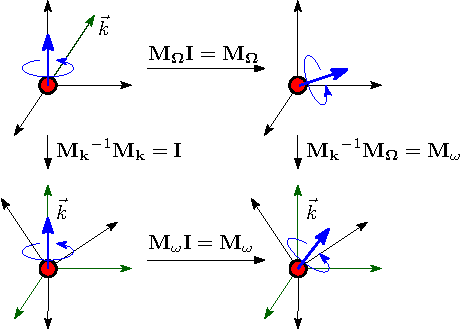
\includegraphics{_figure/rotation_matrix}\caption{Rotation matrices\label{fig:rotation-matrices}}
\par\end{center}%
\end{minipage}%
\begin{minipage}[b][1\totalheight][t]{0.4\columnwidth}%
\begin{center}
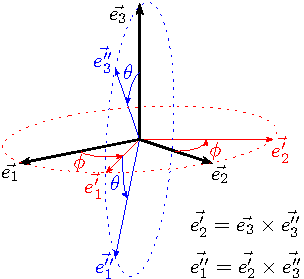
\includegraphics{_figure/rotation_matrix_k}
\par\end{center}
\caption{Rotation to k-frame\foreignlanguage{english}{\label{fig:rotation}}}
%
\end{minipage}
\end{figure}

As shown in fig. \ref{fig:rotation-matrices}, the rotation matrix
for transforming the DCF from the intermolecular coordinates to laboratory
coordinates $\mathbf{\hat{R}}_{\boldsymbol{\omega}}$ can be written
as:
\begin{equation}
\mathbf{\hat{R}}_{\boldsymbol{\omega}}=\mathbf{\hat{R}}_{\mathbf{k}}^{-1}\mathbf{\hat{R}}_{\mathbf{\Omega}}\label{eq:rot-matrix}
\end{equation}
with the rotation matrix related to $\mathbf{k}$ vector:
\begin{equation}
\mathbf{\hat{R}}_{\mathbf{k}}^{-1}=\left[\begin{array}{ccc}
\cos\theta_{k}\cos\phi_{k} & \cos\theta_{k}\sin\phi_{k} & -\sin\theta_{k}\\
-\sin\phi_{k} & \cos\phi_{k} & 0\\
\sin\theta_{k}\cos\phi_{k} & \sin\theta_{k}\sin\phi_{k} & \cos\theta_{k}
\end{array}\right]
\end{equation}

Here we fix $\psi_{k}=0$. As $\theta_{k}$ and $\phi_{k}$ are calculated
from Cartesian coordinates ($k_{x}$, $k_{y}$, $k_{z}$), in the
extreme cases that we cannot define $\theta_{k}$ (for $\left\Vert \mathbf{k}\right\Vert =0$)
and $\phi_{k}$ (for $k_{x}^{2}+k_{y}^{2}=0$), we can arbitrarily
fix those angles to zero.

A faster way to find the rotation matrix of $\mathbf{k}$, avoiding
the evaluation of trigonometric functions, is shown in figure \ref{fig:rotation},
where the matrix can be calculated by the cross products of basis
vectors from $z$ axis and $\mathbf{k}$ vector ($\mathbf{k}=\mathbf{e}_{3}^{''}$):
\begin{equation}
\left[\begin{array}{ccc}
\mathbf{e}_{1}^{''} & \mathbf{e}_{2}^{'} & \mathbf{e}_{3}^{''}\end{array}\right]=\left[\begin{array}{ccc}
\mathbf{e}_{1} & \mathbf{e}_{2} & \mathbf{e}_{3}\end{array}\right]\mathbf{\hat{R}_{k}}=\mathbf{\hat{R}_{k}}
\end{equation}

The two ways to calculate $\mathbf{k}$ differ only in the case of
$\hat{\mathbf{k}}=\left[\begin{array}{ccc}
0 & 0 & -1\end{array}\right]^{T}$, where one is the inverse of the other. This is due to the different
definitions of $\phi_{k}$ ($0$ or $\pi$ when $\overrightarrow{k'_{z}}$
superposes with $\overrightarrow{k_{z}}$) in the two cases. Tests
have shown that it has no influence on the final result of the excess
functional evaluation.

Therefore, the elements of $\mathbf{\hat{R}}_{\boldsymbol{\omega}}$
can be calculated according to eq. (\ref{eq:rot-matrix}):
\begin{align}
\mathbf{\hat{R}}_{\boldsymbol{\omega}} & =\left[\begin{array}{ccc}
u_{x} & v_{x} & w_{x}\\
u_{y} & v_{y} & w_{y}\\
u_{z} & v_{z} & w_{z}
\end{array}\right]\\
 & =\footnotesize\left[\begin{array}{ccc}
\cos\phi\cos\theta\cos\psi-\sin\phi\sin\psi & -\cos\phi\cos\theta\sin\psi-\sin\phi\cos\psi & \cos\phi\sin\theta\\
\sin\phi\cos\theta\cos\psi+\cos\phi\sin\psi & -\sin\phi\cos\theta\sin\psi+\cos\phi\cos\psi & \sin\phi\sin\theta\\
-\sin\theta\cos\psi & \sin\theta\sin\psi & \cos\theta
\end{array}\right]\nonumber 
\end{align}

The angles $\boldsymbol{\omega}$ are thus found as:
\begin{eqnarray}
\cos\theta & = & w_{z}\nonumber \\
\phi & = & \arccos(w_{x}/(w_{x}^{2}+w_{y}^{2})^{\frac{1}{2}})\label{eq:omega}\\
\psi & = & \arccos(-u_{z}/(u_{z}^{2}+v_{z}^{2})^{\frac{1}{2}})\nonumber 
\end{eqnarray}

The resulting angles are between normal intervals, $\cos\theta\in\left[-1,1\right]$,
$\phi\in\left[0,2\pi\right]$. As water possesses $\mathrm{C}_{2v}$
symmetry, we take $\psi\in\left[0,\pi\right]$. 

\textcolor{red}{(Expliquer ici -à noiveau– pourquoi tu as besoin de
faire des interpolations: grille plus fine pour om dans c(k,om\_1,om\_2)
et pour chaque (k,Omega) on doit trouver le om corerspondant.)}

The interpolation of these found angles to the intermolecular grid
can be done with different orders: zeroth order interpolation, which
directly takes the nearest point, or linear interpolation.

\subsection{Zero-order interpolation of DCF\label{subsec:Zero-order-interpolation-of}}

At this order, for each possible value of $\mathbf{k}$ and $\mathbf{\Omega}$,
the corresponding $\cos\theta$ and $\psi$ which relate to only one
solvent molecule are stored as an index (single precision integer),
which gives the nearest angle in a pre-defined table:
\begin{equation}
\begin{array}{l}
i_{\cos\theta}=\left\lfloor (\cos\theta+1)(n_{\cos\theta}/2)\right\rfloor +1\\
i_{\psi}=\mathrm{mod}(\left\lfloor \psi(n_{\psi}/\pi)\right\rfloor ,n_{\psi})+1
\end{array}
\end{equation}
where $\left\lfloor f\right\rfloor $ is the floor function. For the
angle $\phi$ which relate to two solvent molecules, the operation
$\phi=\phi_{1}-\phi_{2}$ introduces a double error when integer indices
are used, as shown in figure \ref{fig:diff_phi}.

\begin{figure}[h]
\begin{centering}
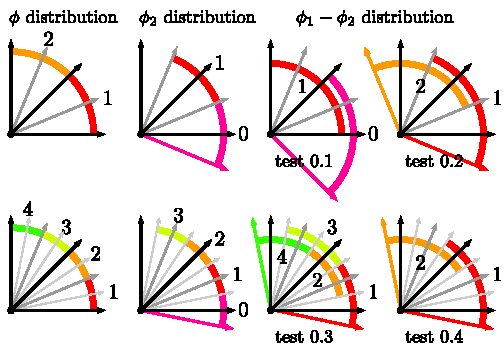
\includegraphics{_figure/diff_phi}
\par\end{centering}
\caption[$\phi_{1}-\phi_{2}$ distribution]{$\phi_{1}-\phi_{2}$ distribution: Test 0.1 is the direct subtraction
of $\phi$ established in the same way with $\theta$ and $\psi$,
as shown in the top first schema. Test 0.2 tabulates $\phi_{2}$ by
taking the nearest point in another manner, as shown in the second
schema. In test 0.3-0.4, all $\phi$ or only $\phi_{2}$ is doubled.\label{fig:diff_phi}}
\end{figure}

In the actual implementation, as an integer takes 4 bytes and a real
takes 8 bytes, there is no profit to tabulate $\phi$ in integer two
times, thus $\phi$ is stored directly in real.

\subsection{Linear interpolation of DCF\label{subsec:Linear-interpolation-of}}

At this order, $\boldsymbol{\omega}(\mathbf{k},\mathbf{\Omega})$
is stored in double precision. All angles are stored in real type,
and the corresponding DCF is calculated as
\begin{equation}
c(\omega)=w_{0}c(\omega_{0})+w_{1}c(\omega_{1})
\end{equation}
where $w_{0}=\frac{\omega_{1}-\omega}{\omega_{1}-\omega_{0}}$ and
$w_{1}=\frac{\omega-\omega_{0}}{\omega_{1}-\omega_{0}}$. Here $\omega$
is one of the 5 dimensions in $\tilde{\boldsymbol{\omega}}(\mathbf{k},\mathbf{\Omega_{1}},\mathbf{\Omega_{2}})\equiv(\cos\theta_{1},\cos\theta_{2},\phi,\psi_{1},\psi_{2})$,
$\omega_{0}$ and $\omega_{1}$ are the 2 nearest value points, while
other variables are fixed. If we express the weight for each dimension
as $w_{n_{i}}^{i}$ where $i=1,2,3,4,5$ is the $i$th variable, the
total equation with 5 variables is:
\begin{equation}
c(\tilde{\boldsymbol{\omega}})=\left[\sum_{n_{1}=0}^{1}\sum_{n_{2}=0}^{1}\sum_{n_{3}=0}^{1}\sum_{n_{4}=0}^{1}\sum_{n_{5}=0}^{1}\left(\prod_{i}^{5}w_{n_{i}}^{i}c(\tilde{\boldsymbol{\omega}}_{n_{1},n_{2},n_{3},n_{4},n_{5}})\right)\right]\label{eq:interpolation}
\end{equation}

These two equations are available for both interpolation and extrapolation,
where the latter applies, e.g., for $\cos\theta_{1}$ and $\cos\theta_{2}$. 

An error evaluation of these two strategies of interpolation is shown
in appendix \ref{chpt:error-evaluation-interpolation-DCF}. Results
demonstrate that the linear interpolation scheme is absolutely essential.
On the other hand, as seen in eq. (\ref{eq:interpolation}), it is
computationally much more expensive than the simple histogram scheme
as it requires $2^{5}=32$ times the number of operations.

\section{Direct calculation of DCF from rotational invariant projections}

Another strategy to calculate $\hat{c}(\mathbf{k},\mathbf{\Omega_{1}},\mathbf{\Omega_{2}})$
is to use the DCF expressed in terms of rotational invariant projections,
which takes far less memory than in the intermolecular form thanks
to their angular independence and symmetric properties. 

\subsection{Using projections in form of $\hat{c}_{\mu\nu}^{mnl}(k)$\label{subsec:Using-projections-in}}

As described by Blum \citep{Blum_I,Blum_II}, $\hat{c}(\mathbf{k},\mathbf{\Omega_{1}},\mathbf{\Omega_{2}})$
can be expanded as
\begin{equation}
\hat{c}(\mathbf{k},\mathbf{\Omega_{1}},\mathbf{\Omega_{2}})=\sum_{mnl\mu\nu}\hat{c}_{\mu\nu}^{mnl}(k)\Phi_{\mu\nu}^{mnl}(\mathbf{\hat{k}},\mathbf{\Omega_{1}},\mathbf{\Omega_{2}})
\end{equation}
where $\Phi_{\mu\nu}^{mnl}(\mathbf{\hat{k}},\mathbf{\Omega_{1}},\mathbf{\Omega_{2}})$
is the rotational invariant that depends on both the spatial and angular
coordinates of the two particles (detailed in appendix \ref{chpt:rotational-invariant-expansion}).

For projections of order $n_{\mathrm{max}}=1$, the DCF can be expressed
in very simple form. Only 4 projections $\hat{c}^{mnl}(k)$ are independent:
$\hat{c}_{\mathrm{S}}\equiv\hat{c}^{000}$, $\hat{c}_{\mathrm{\Delta}}\equiv\hat{c}^{110}$,
$\hat{c}_{\mathrm{D}}\equiv\hat{c}^{112}$ and $\hat{c}_{+}\equiv\hat{c}^{011}=-\hat{c}^{101}$,
with the corresponding rotational invariants expressed below both
in laboratory and intermolecular frames \textcolor{red}{(il faut définir
ici OM\_1 et OM\_2 comme des vecteurs d'orientation !)}
\begin{align}
\Phi^{000} & =1\nonumber \\
\Phi^{011} & =i\mathbf{k}\cdot\mathbf{\Omega}_{1}=i\cos\theta_{1}\nonumber \\
\Phi^{101} & =i\mathbf{k}\cdot\mathbf{\Omega}_{2}=i\cos\theta_{2}\nonumber \\
\Phi^{110} & =-\sqrt{3}\mathbf{\Omega}_{1}\cdot\mathbf{\Omega}_{2}=-\sqrt{3}(\sin\theta_{1}\sin\theta_{2}\cos\phi_{12}+\cos\theta_{1}\cos\theta_{2})\nonumber \\
\Phi^{112} & =\sqrt{\frac{3}{10}}\left[3\mathbf{(\mathbf{k}\cdot\mathbf{\Omega}_{1})(\mathbf{k}\cdot\mathbf{\Omega}_{2})-\Omega}_{1}\cdot\mathbf{\Omega}_{2}\right]\\
 & =\sqrt{\frac{3}{10}}\left(2\cos\theta_{1}\cos\theta_{2}-\sin\theta_{1}\sin\theta_{2}\cos\phi_{12}\right)\nonumber 
\end{align}

To express the DCF at higher orders, the number of FE needed for $\Phi_{\mu\nu}^{mnl}(\mathbf{\hat{k}},\mathbf{\Omega_{1}},\mathbf{\Omega_{2}})$
becomes huge and the DCF should be calculated in intermolecular frame
as indicated above.

\subsection{Using projections in form of $\hat{c}_{\mu\nu,\chi}^{mn}(k)$\label{subsec:Using-projections-in-1}}

Compared to the expression of $\Phi_{\mu\nu}^{mnl}(\mathbf{\hat{k}},\mathbf{\Omega_{1}},\mathbf{\Omega_{2}})$
in laboratory frame (eq. (\ref{eq:definition_rot_invar}) in appendix
\ref{chpt:rotational-invariant-expansion}), its intermolecular form
has far fewer terms (eq. (\ref{eq:phi_local}) in appendix \ref{chpt:rotational-invariant-expansion}),
such that
\begin{equation}
\hat{c}(k,\boldsymbol{\omega_{1}},\boldsymbol{\omega_{2}})=\frac{1}{2l+1}\sum_{mn\mu\nu\chi}\hat{c}_{\mu\nu,\chi}^{mn}(k)r_{\chi\mu}^{m}(\theta_{1})r_{-\chi\nu}^{n}(\theta_{2})e^{-i\chi(\phi_{12}\equiv\phi_{1}-\phi_{2})}e^{-i\mu\psi_{1}}e^{-i\nu\psi_{2}}\label{eq:dcf-exact}
\end{equation}
where $r$ is the generalized Legendre polynomial,$m,n\leq n{}_{\mathrm{max}}$,
$\left|\mu\right|\leq m$, $\left|\nu\right|\leq n$, and $\chi\in\left[-\mathrm{min}(m,n),\mathrm{min}(m,n)\right]$.

$r_{\chi\mu}^{m}(\theta)$, $e^{-i\chi\phi}(\phi)$ and $e^{-i\mu\psi}(\psi)$
can be separately pre-tabulated for each given $\mathbf{k}$, to avoid
double evaluation of each term.

E.q. (\ref{eq:dcf-exact}) replaces the interpolation of eq. (\ref{eq:interpolation})
by an exact formula and it requires the projections $\hat{c}_{\mu\nu,\chi}^{mn}(k)$
to be stored in memory rather than the full angular representation
$\hat{c}(k,\boldsymbol{\omega_{1}},\boldsymbol{\omega_{2}})$. It
also requires the passage from orientations in laboratory frame to
orientations in intermolecular frame, i.e. use of the formulae (\ref{eq:omega})
for each $\mathbf{k}$ vector.
